\documentclass{standalone}
\usepackage{tikz}
\usepackage{pgfplots}
\pgfplotsset{compat=1.17}

\begin{document}

% Bode Magnitude Plot
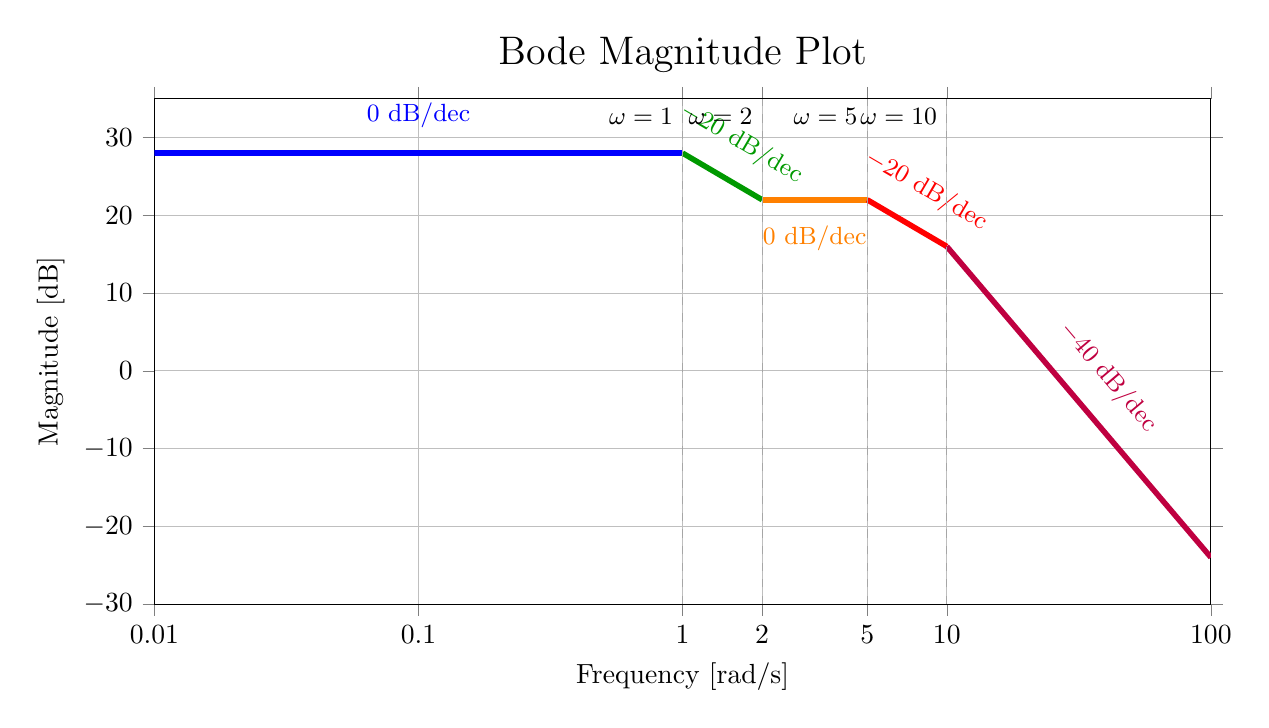
\begin{tikzpicture}
    \begin{semilogxaxis}[
        width=15cm,
        height=8cm,
        xlabel={Frequency [rad/s]},
        ylabel={Magnitude [dB]},
        xmin=0.01, xmax=100,
        ymin=-30, ymax=35,
        xtick={0.01,0.1,1,2,5,10,100},
        xticklabels={0.01,0.1,1,2,5,10,100},
        ytick={-30,-20,-10,0,10,20,30},
        grid=both,
        minor grid style={gray!20},
        major grid style={gray!50},
        tick align=outside,
        xmajorgrids,
        ymajorgrids,
        xlabel near ticks,
        ylabel near ticks,
        title={\Large Bode Magnitude Plot},
        ]

        % Plotting the magnitude plot with creative coloring

        % Segment 1: From 0.01 to 1 rad/s (0 dB/decade)
        \addplot[
            color=blue,
            line width=2pt,
        ] coordinates {
            (0.01,28)
            (1,28)
        } node[pos=0.5, above, color=blue, yshift=5pt] {\small $0$ dB/dec};

        % Segment 2: From 1 to 2 rad/s (-20 dB/decade)
        \addplot[
            color=green!60!black,
            line width=2pt,
        ] coordinates {
            (1,28)
            (2,22)
        } node[pos=0.5, above, sloped, color=green!60!black, yshift=5pt] {\small $-20$ dB/dec};

        % Segment 3: From 2 to 5 rad/s (0 dB/decade)
        \addplot[
            color=orange,
            line width=2pt,
        ] coordinates {
            (2,22)
            (5,22)
        } node[pos=0.5, below, color=orange, yshift=-5pt] {\small $0$ dB/dec};

        % Segment 4: From 5 to 10 rad/s (-20 dB/decade)
        \addplot[
            color=red,
            line width=2pt,
        ] coordinates {
            (5,22)
            (10,16)
        } node[pos=0.5, above, sloped, color=red, yshift=5pt] {\small $-20$ dB/dec};

        % Segment 5: From 10 to 100 rad/s (-40 dB/decade)
        \addplot[
            color=purple,
            line width=2pt,
        ] coordinates {
            (10,16)
            (100,-24)
        } node[pos=0.5, above, sloped, color=purple, yshift=5pt] {\small $-40$ dB/dec};

        % Add the break frequencies as vertical dashed lines
        \addplot[dashed, color=gray!70] coordinates {(1,-30) (1,35)};
        \addplot[dashed, color=gray!70] coordinates {(2,-30) (2,35)};
        \addplot[dashed, color=gray!70] coordinates {(5,-30) (5,35)};
        \addplot[dashed, color=gray!70] coordinates {(10,-30) (10,35)};

        % Annotate break frequencies
        \node[anchor=north east, color=black] at (axis cs:1,35) {\small $\omega=1$};
        \node[anchor=north east, color=black] at (axis cs:2,35) {\small $\omega=2$};
        \node[anchor=north east, color=black] at (axis cs:5,35) {\small $\omega=5$};
        \node[anchor=north east, color=black] at (axis cs:10,35) {\small $\omega=10$};

    \end{semilogxaxis}
\end{tikzpicture}
\end